\subsection{Diagrammi delle classi del Model}
			\subsubsection{Package Database}
			\begin{center}
				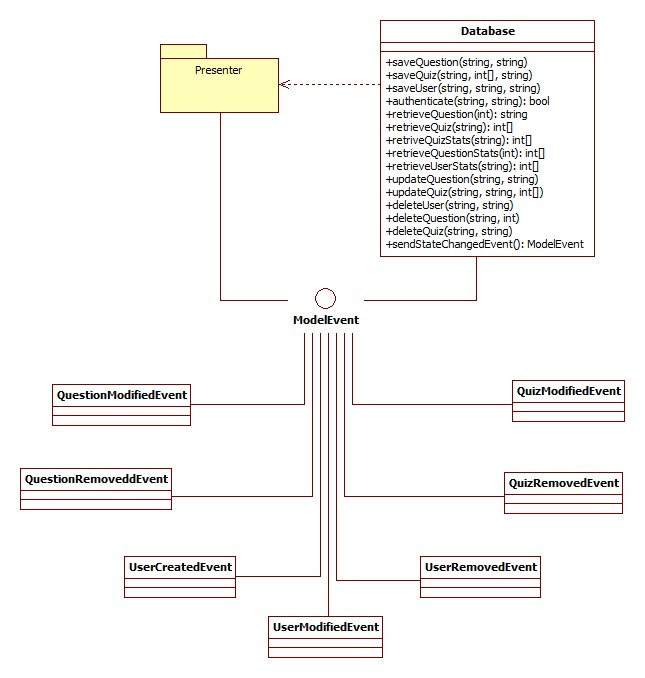
\includegraphics[scale=0.5]{../images/Database.jpg}
			\end{center}
			\subsubsubsection{Classe QuizManager}
			\begin{itemize}
		    	\item\textbf{Funzione del componente:} la classe permettera' l'inserimento, la lettura e la rimozione di questionari all'interno della collezione
			\item\textbf{Relazioni d'uso di altri componenti:} interagisce con la ViewModel, gestendo le richieste per inserire, modificare o eliminare quiz
			\end{itemize}
			\subsubsubsection{Classe QuestionManager}
			\begin{itemize}
		    	\item\textbf{Funzione del componente:} la classe permettera' l'inserimento, la lettura e la rimozione di singoli quesiti all'interno della collezione
			\item\textbf{Relazioni d'uso di altri componenti:} interagisce con la ViewModel, gestendo le richieste per inserire, modificare o eliminare quesiti
			\end{itemize}
			
			\subsubsection{Package Parser}
			\begin{center}
				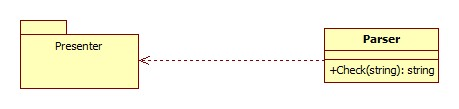
\includegraphics[scale=0.6]{../images/Parser.jpg}
			\end{center}
 			\subsubsubsection{Classe Parser}
 			\begin{itemize}
		    	\item\textbf{Funzione del componente:} controlla che il testo fornito risulti corretto secondo la sintassi QML
			\item\textbf{Attivita' svolte e dati trattati:} il Parser controlla che il testo fornito in input rispetta la sintassi QML e fornisce in caso di errore un messaggio avvertendo l'utente di dove si trova l'errore e la tipologia
			\end{itemize}
			
			\subsubsection{Package Statistics}
			\begin{center}
				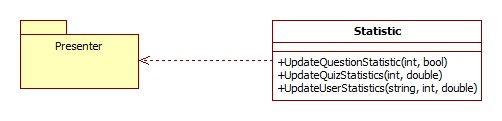
\includegraphics[scale=0.4]{../images/Statistics.jpg}
			\end{center}
 			\subsubsubsection{Classe Statistics}
 			\begin{itemize}
		    	\item\textbf{Funzione del componente:} questa classe fornisce funzionalita' per il raccoglimento delle statistiche sulle prestazioni degli utenti del sistema
			\item\textbf{Attivita' svolte e dati trattati:} la classe aggiornera' le statistiche relative ai quesiti, questionari ed utenti.
			Per i quesiti verranno indicati il numero di volte che e' stato proposto e il numero di risposte corrette.
			Per i questionari verranno indicati le valutazioni medie ottenute dagli utenti e il numero di volte che e' stato proposto.
			Per gli utenti verranno indicati la valutazione migliore e la media dei tentativi eseguiti su singolo quiz
			\end{itemize}
			
			\subsubsection{Package Publishers}
			\begin{center}
				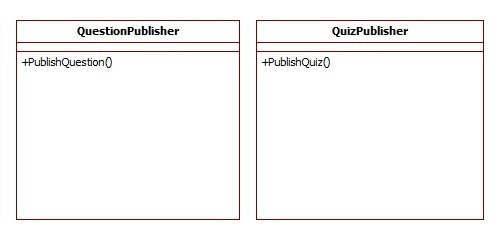
\includegraphics[scale=0.9]{../images/Publishers.jpg}
			\end{center}
			\subsubsubsection{Classe QuizPublisher}
			\begin{itemize}
				\item\textbf{Funzione del componente:} questa classe fornisce funzionalita' per la pubblicazione dei quiz
				\item\textbf{Attivita' svolte e dati trattati:} questa classe permette ad un utente di accedere alla collezione dei quiz
			\end{itemize}
			\subsubsubsection{Classe QuestionPublisher}
			\begin{itemize}
				\item\textbf{Funzione del componente:} questa classe fornisce funzionalita' per la pubblicazione dei quesiti
				\item\textbf{Attivita' svolte e dati trattati:} questa classe permette ad un utente di accedere alla collezione dei quesiti
			\end{itemize}
			\newpage